\subsubsection{TIMELY has no fixed point, is inherently unstable with
unpredictable fairness}
We attempted to perform the same analysis for TIMELY that we performed for DCQCN
in the previous section.  The first step in performing the analysis is to obtain
the fixed point of the system.  However, the way the TIMELY algorithm is
implemented, it has \emph{no fixed point}. The implication is that the queue
length never converges, nor do the sending rates of the flows. The system
operates in limit cycles, always oscillating. Moreover, while the system is
oscillating, there are \emph{infinite} solutions for the sending rates of the
flows that satisfy the fluid equations at any point. So, even if we can limit
the magnitude of the limit cycles by choosing parameters carefully, we can make
no claims on the fairness of the protocol since the system could be operating at
any of those infinite solutions. We first show that it has no fixed point.

\begin{thm}[No fixed point for TIMELY] 
\label{thm:nofixed}
Under the model described by Figure~(\ref{tab:timely_param}), the system has no
fixed points.
\end{thm}
\begin{proof}
We prove the result by contradiction. At the fixed point, all
differential equations converge to 0. Thus
\begin{eqnarray*}
\frac{dq}{dt} & =& 0 
\end{eqnarray*}  and 
\begin{eqnarray*} \sum_{i} R_i(t) & = & C \end{eqnarray*}
Now, , either $g > 0$ or $g  \le 0$. If $g \ne 0$, then since 
\begin{eqnarray*}
\frac{{dg}}{{dt}} & = & \frac{\alpha }{{\tau *}}( - g(t) + \frac{{q(t
                        - \tau ') - q(t - \tau ' - \tau
                        *)}}{{C*{D_{\min RTT}}}})\\
& = &  -\frac{\alpha }{{\tau *}} g(t)  \\
& \ne & 0 
\end{eqnarray*}
Thus $ g = 0$ for the derivative of  $g$ to converge to 0. Then we obtain
\begin{eqnarray*}
 \frac{dR_i}{dt} & = & \frac{\delta }{{\tau *}}\\
& \ne & 0
\end{eqnarray*}
Thus, all derivaties cannot be simultaneously 0 and the system
described by Figure~(\ref{tab:timely_param}) has no fixed point.
\end{proof}

% In fixed point analysis, we identify the point at which the derivatives of the
% various quantities in the fluid model become 0.  Setting $\tfrac{dq}{dt} = 0$,
% we obtain $\sum_{i} R_i(t) = C$. Next, we have two possibilities, either $g > 0$
% or $g  \le 0$. If $g$ takes a non-zero value, then $\tfrac{dg}{dt}$ cannot be 0,
% as the second term in Equation~\ref{eq:timely_g} needs to be 0 for
% $\tfrac{dq}{dt}$ to be 0. Thus, we require $g$ to be 0 at the fixed point.
% However, from Equation~\ref{eq:timely_r}, we see that if $g = 0$,
% $\tfrac{dR_i}{dt}$ \emph{cannot} be 0 since $\delta$ is not 0. Thus, from the
% protocol description, the fluid model has no fixed points as the derivatives
% cannot be simultaneously 0 and thus the (fluid) system never stabilizes to any
% value.
We modify the fluid model very slightly, by moving the equality condition
to the term involving $g$, and have a modified fluid model that looks like the
following:

\begin{equation}
\frac{{dR_i}}{{dt}} = \left\{ \begin{array}{ll}
\frac{\delta }{{\tau *}}, & q(t - \tau ') < C*{T_{low}}\\
\frac{\delta }{{\tau *}}, & g < 0\\
 - \frac{{g\beta }}{{\tau *}}R(t), & g \ge 0\\
 - \frac{\beta }{{\tau *}}(1 - \frac{{C*{T_{high}}}}{{q(t - \tau ')}})R(t), & q(t - \tau ') > C*{T_{high}}
\end{array} \right.\\
\label{eq:timely_r_modified}
\end{equation}

\begin{figure*}[t]
\center
\subfigure[Both flows start at time 0 at 5Gbps] { 
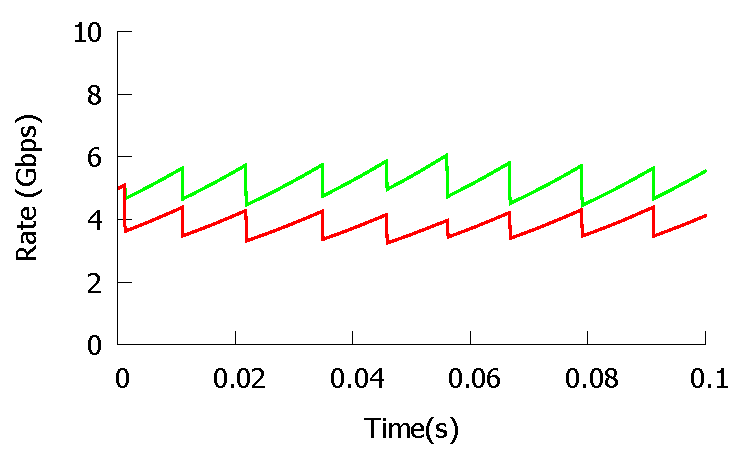
\includegraphics[width=0.3\textwidth]{figures/timely_stability_2f55.pdf}
}
\subfigure[Both start at 10Gbps, one starts 10ms late] { 
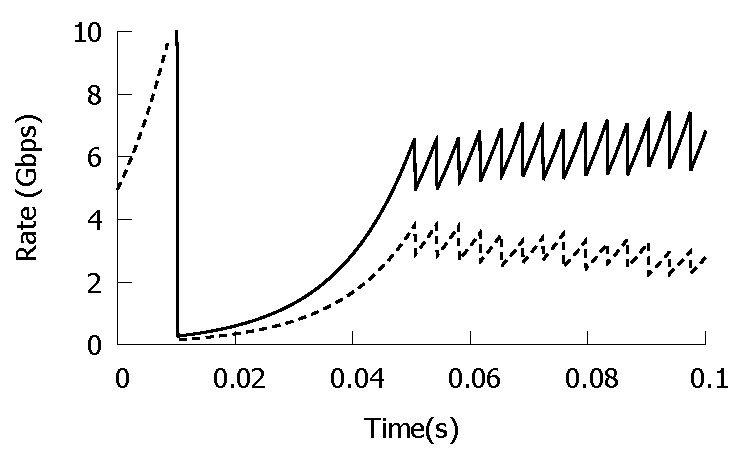
\includegraphics[width=0.3\textwidth]{figures/timely_stability_2ftime.pdf}
}
\subfigure[Both start at time 0, one at 7Gbps, other at 3Gbps] { 
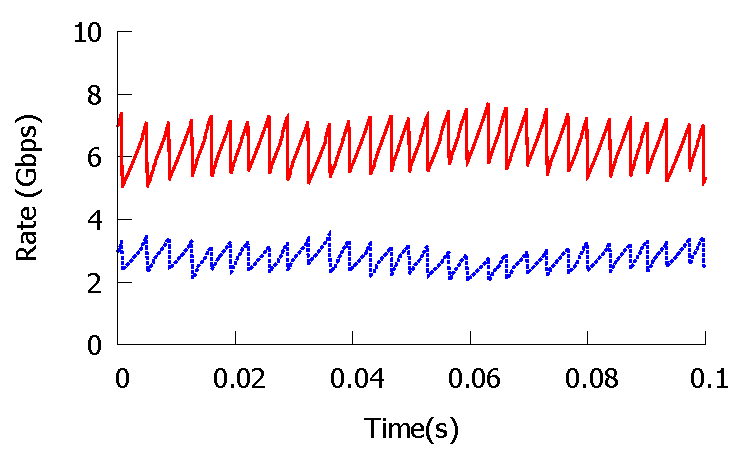
\includegraphics[width=0.3\textwidth]{figures/timely_stability_2f73.pdf}
}
\caption{Performance of two TIMELY flows under different starting conditions}
\label{fig:timely_unstable}
\end{figure*}

\para{Infinite fixed points for modified model:}
Practically, this change does not make much of a difference and it is
in fact how the protocol behaves, as we verify via simulations. With this
modification, we can now obtain the condition that with $g =0$, $\tfrac{dq}{dt}
= 0$, $\tfrac{dg}{dt} = 0$ and $C*T_{low} < q < C*T_{high}$. However, now we run
into the issue that TIMELY moves from zero fixed points to \emph{infinite} fixed
points.
\begin{thm}[Infinite fixed points]
The system described by Figure~(\ref{tab:timely_param}) with a
modification introduced in Equation~\ref{eq:timely_r_modified} has
infinite fixed points
\end{thm}
\begin{proof}
 To obtain 

$$\frac{dg}{dt} =0$$ we need $g = 0$ and
$$\frac{dq}{dt} = 0$$ Any value of $q$ such that $C*T_{low} < q <
C*T_{high}$ makes $$\frac{dR_i}{dt} = 0$$ for any value of $R_i$ as
long as $\sum_{i} R(t) =  C$ and hence $q$ have infinitely many fixed
points. 
%As a
%practical matter, those values are in fact finitely many and we can live with
%the fact that $q$ will remain between $C*T_{low}$ and $C*T_{high}$. What is more
%troubling is 
%From Equation~\ref{eq:timely_q}. At the
%fixed point $$\frac{dq}{dt} = 0$$ as long as $\sum_{i} R(t) =  C$. From
%Equation~\ref{eq:timely_r_modified}, we know that as long as $q$ is between the
%thresholds $ C*{T_{low}}$ and $C*{T_{high}}, g=0$, $\tfrac{dR_i}{dt} = 0$. Thus, the individual rates can
%take on \emph{any} value, as long as they sum up to $C$. At $q = C*{T_{high}}$, any value of $R_{i}$ will make the
%derivative 0. Thus, $q$ has infinite fixed points, and at each of
%those infinite fixed points, $R_i$ can take any value as long as
%$\sum_{i} R(t) =  C$. 
$q$ cannot converge to any value outside of the
thresholds $ C*{T_{low}}$ and $C*{T_{high}}$ as that would
imply $$\frac{dR_i}{dt} \ne 0$$.
\end{proof}
There is no requirement that at the fixed point $R_i = \tfrac{C}{N}$. In
fact, $\tfrac{R_{i}}{R_{j}}, i \ne j$ is not even bounded, so we cannot make any
claims on the fairness of TIMELY. Thus the fixed point of TIMELY is entirely
unpredictable and this is a fundamental flaw of the protocol. This is borne out
by the simulation results shown in Figure~\ref{fig:timely_unstable}, where we
only change the start time and initial rates of two flows, keeping everything
else constant, and we end up in completely different operating regimes.


We next prove another result that gives a fundamental tradeoff between
fairness and guaranteed delay for protocols that
rely on delay measurements at the end points to implement congestion
control.
\begin{thm}[Fairness/Delay tradeoff]
For congestion control mechanisms that relay purely on end to end
delay measurements, you can either have fairness or a guaranteed delay
bound, but not both simultaneously.
\end{thm}
\begin{proof}
Suppose you have N flows sharing a link of capacity $C$. Then every flow
should distributedly arrive at a rate $C/N$ and the flows need to know
this $N$. If we use end to end delay as the only signal, then this delay
has to carry information about $N$ and hence the converged delay
depends on $N$ and cannot be guaranteed independently. Conversely, if we implement a guaranteed delay congestion
control scheme at the end points, they
will converge to any rate $R_i$ such that $\sum_{i=0}^{N}R_i = C$
making the derivative of measured delay 0 and the actual delay equal
to the guarantee. Since the guarantee is set independent of $N$, the
actual delay contains no information on N and 
thus such a scheme cannot ensure fairness.
\end{proof}


% that we proposed, guarantees a tunable delay, and we showed the queue converges to that delay under all sorts of varying conditions and the flows converge to a fair share. %The key to that is that the feedback, p, is computed and relayed in a centralized manner by the router. If each flow computes the feedback independently, and they keep getti%ng this same signal (the common delay which they are trying to tune independent of the number of flows), then the flows *cannot* estimate N, and hence cannot converge to %C/N and you can’t have fairness.

%%% Local Variables:
%%% mode: latex
%%% TeX-master: "main"
%%% End:
